\subsection{Методы геномного анализа в исследовании структуры хроматина}
% сделать на основе https://docs.google.com/document/d/1GcTfefw2HnJGGnGmaJP5w2JN1Jy8X2EyCjyOlxEbagU/edit?usp=sharing

    Для определения наличия физического контакта между последовательностями ДНК в трехмерной структуре генома были разработаны методы семейства -С: 3С, 4С, 5С, Hi-C \cite{fraser_overview_2015}. Эти методы основаны на химическом ``сшивании'' контактирующих в хроматине участков, фрагментации ДНК с образованием ``сшитых'' пар, лигирования фрагментов в этих парах с образованием гибридных молекул ДНК, детекции гибридных молекул (обнаружение молекулы, состоящей из последовательности А и последовательности В, говорит о физическом контакте локусов этих последовательностей в ДНК).
    Существует понятие ``разрешения'' метода Hi-C (см. Таблицу \ref{tab:p1:hic}). Его можно определить как минимальное расстояние (в парах оснований) между участками, на котором они отображаются на тепловую карту в разные ее точки (пиксели). Величина разрешения зависит от величины фрагментов, на которые рестриктазы разрезают ДНК (то есть от особенностей используемых рестриктаз, размеров и встречаемости в геноме их сайтов рестрикции), и от размера бина, выбираемого на стадии обработки данных Hi-C, но не полностью произвольного: для получения тепловой карты, адекватно представляющей трехмерную структуру изучаемого генома, необходимо выбирать размеры бинов из определенного диапазона, зависящего от размеров хромосом, глубины секвенирования и качества NGS-библиотеки \cite{pal_hi-c_2019}. От разрешения метода Hi-C зависит то, какие структуры в хроматине он может выявить. Оригинальный протокол метода, описанный в статье 2009 года \cite{lieberman-aiden_comprehensive_2009}, позволял достичь разрешения 4kb и выявлял, соответственно, в трехмерной структуре генома компартменты A и B (соответствующие активному и неактивному хроматину). В протоколах Hi-C, разработанных позже, достигалось, благодаря использованию других рестриктаз, большее разрешение - до одной килобазы. Это позволяло обнаружить так называемые топологически ассоциированные домены (ТАДы) \cite{dixon_topological_2012} и взаимодействия конкретных последовательностей друг с другом - то есть, физические контакты регуляторных элементов с регулируемыми ими генами, реализованные, как полагают современные исследователи, запетливанием ДНК. Однако этих разрешающих способностей все равно не достаточно, чтобы изучить супрануклеосомный уровень, на котором ранее предполагалось существование 30-нанометровой фибриллы \cite{pal_hi-c_2019}.
    
    Пролить свет на этот уровень смог метод Micro-C — модификация метода Hi-C, предполагающая использование на этапе фрагментации ДНК микрококковой нуклеазы, которая уничтожает линкерные участки, оставляя одни  нуклеосомы (этот метод можно рассматривать как синтез метода позиционирования нуклеосом с помощью микрококковой нуклеазы - MNase-seq \cite{cui_genome-wide_2012} - и Hi-C \cite{hsieh_mapping_2015}. Это позволяет оценивать частоту взаимодействия отдельных нуклеосом друг с другом, то есть разрешение метода достигает неизученного супрануклеосомного уровня (между 200bp и 4kb), устраняя так называемый ``пробел в разрешении'' (resolution gap). Интересно, что метод Micro-C тоже не обнаружил 30-нанометровую фибриллу, еще раз доказав необходимость дальнейших исследований структуры хроматина супрануклеосомного уровня. В работе, в которой впервые был предложен метод Micro-C, изучался геном дрожжей - \textit{S. cerevisiae}. 
    
    Параллельно Micro-C был разработан другой метод Hi-C высокого разрешения - in situ DNase Hi-C. С его помощью можно получить данные с разрешением около 1kb \cite{ramani_mapping_2016}. Однако этот метод, основанный на использовании фермента DNase I, неспецифически фрагментирующего ДНК на тетрануклеотиды, не является конкурентным для Micro-C в области изучения супрануклеосомной структуры хроматина, так как не уничтожает линкерную ДНК и, соответственно, не позволяет в отличие от Micro-C простым способом получить данные о частоте взаимодействия нуклеосом друг с другом. 
    Сам протокол Micro-C модифицировался после его изобретения. Примером могут служить работы \cite{hsieh_micro-c_2016} и \cite{ohno_sub-nucleosomal_2019}, в которых были впервые представлены модификации Micro-C:  Micro-C XL и Hi-Co, соответственно. Micro-C XL - метод, позволяющий получить качественные данные в мононуклеосомном разрешении, это достигается путем снижения шума за счет изоляции нерастворимого хроматина и использования помимо формальдегида длинных сшивающих агентов (кросслинкеров) - например, DSG и EGS. Метод Hi-Co специфичен тем, что с его помощью можно определить ориентацию нуклеосом (``O''  в названии - от Orientation). Это достигается с помощью особой биоинформатической обработки и использования не просто секвенирования спаренных концов, а секвенирования спаренных концов с тэгами (PET - paired-end tags \cite{fullwood_next-generation_2009}).
    
    \begin{table}[p]
\caption{Увеличение разрешения Hi-C подобных методов, благодаря использованию менее специфичных рестриктаз.}
	\label{tab:p1:hic}	
	\begin{tabularx}{\textwidth} { 
  | >{\raggedright\arraybackslash}X 
  | >{\centering\arraybackslash}X 
  | >{\raggedleft\arraybackslash}X 
  | >{\raggedleft\arraybackslash}X |}
  \hline
Протокол Hi-C & Рестриктазы & Сайты рестрикции & Размер сайта рестрикции\\
	\hline

Классический (Lieberman-Aiden et al., 2009) & HindIII, NcoI & AAGCTT, CCATGG & 6 пн \\
\hline
Sexton et al., 2012, Rao et al., 2014 & Dpn-II & GATC & 4 пн \\
\hline
COLA (Darrow et al., 2016) & CviJI & RCGY, R=A/G, Y=C/G & 3 пн \\
\hline
Micro-C (Hsieh et al., 2016) & MNase & Отсутствует. Эндо/экзо нуклеаза, почти полностью уничтожает линкерные участки ДНК &  - \\
\hline
in situ DNAse Hi-C (Ramani et al., 2016) & DNAse I & Отсутствует. Режет ДНК на тетранукеотиды & -  \\
\hline
\end{tabularx}
	 
\end{table}
    
    Следует отметить, что все методы -C являются статистическими и вероятностными, приблизительно оценивающими частоту взаимодействия большого количества фрагментов ДНК. Для получения биологически значимой информации с помощью метода Hi-C вообще и, в частности Micro-C, необходим тщательный биоинформатический анализ матриц взаимодействия: фильтрация  и нормализация данных, учет того — использовалась в методе клеточная популяция или единичная клетка (Single-Cell Hi-C/Micro-C \cite{nagano_single-cell_2013}). Для изучения супрануклеосомной структуры хроматина с помощью Micro-C необходимо дополнительно прибегнуть к его молекулярному моделированию с учетом последних достижений в вычислительной биофизики.

\begin{figure} [h!]
    \centering
    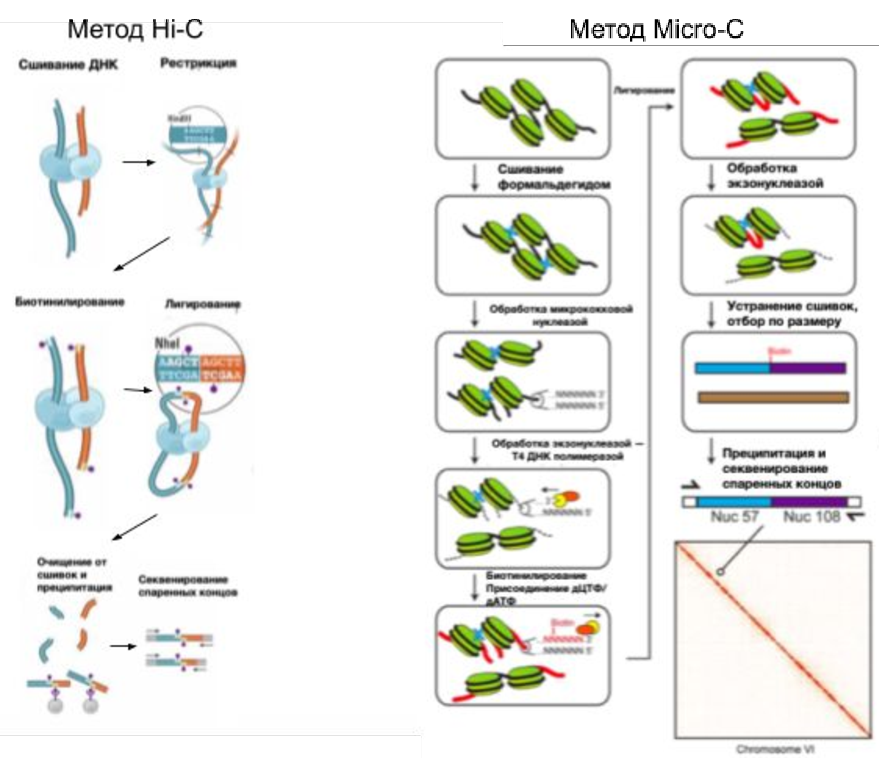
\includegraphics [width=\textwidth]{images/p1/part1_5_genome/p1_5_genome_f5.pdf}
    \caption[Методы ``захвата конформации хроматина''.]{Методы ``захвата конформации хроматина'' (chromatin conformation capture), сравнение Hi-C и Micro-C. Адаптировано из \cite{lieberman-aiden_comprehensive_2009} и \cite{hsieh_mapping_2015}.}
    \label{fig:p1_5_genome:f5}
\end{figure}


    Появление методов секвенирования нового поколения дало огромное преимущество большинству методов эпигеномики, позволяющим получать данные о местах расположения нуклеосом, в том числе с гистоновыми вариантами и с определенными пост-трансляционными метками гистонов. 

    Метод MNase-seq позволяет получить данные о расположении единичных нуклеосом. В методе используется микрококковая нуклеаза, которая обладает экзо- и эндонуклеазными активностями. После работы нуклеазы, нуклеосомальная ДНК освобождается от гистонов и секвенируется. Далее прочтения картируются на референсный геном.       На данный момент в публичном доступе накоплено большое количество экспериментальных наборов данных для клеток разных организмов и из разных тканей человека (110 наборов данных по данным сайта \url{https://generegulation.org/nucleosome-positioning-database/}).
    К основным проблемам использования методов Mnase-seq относится огромное количество получаемых с одного эксперимента прочтений - порядка 200-400 млн для клеточных линий человека. Для достижения оптимального разрешения позиционирования нуклеосом в человеческих клетках для сравнения здоровых и больных требуется порядка 1-4 млрд прочтений \cite{teif_nucleosome_2016}. Обычно эксперименты MNase-seq выполняют на нескольких тысячах клеток, такой усредненный нуклеосомальный профиль характеризует ансамбль клеток, а не частные состояния клеток. Специализированная база данных NucMap включает 798 экспериментальных наборов данных MNase-seq из 477 образцов для 15 видов живых организмов \cite{zhao_nucmap:_2019}. Для дрожжей существует метод СС-seq, позволяющий определять позиционирование нуклеосом с большей точностью, чем MNase-seq \cite{brogaard_map_2012}. Суть метода в ведении специальной мутации в гистоны, в результате которой вблизи центра нуклеосомы появляется остаток цистеина. Боковая цепь цистеина используется для реакции со специальными химическими агентами, которые разрезают ДНК в центре нуклеосомы. Далее методами секвенирования определяется положение разреза и, следовательно, центра нуклеосомы.
    Методы ChIP-seq осуществляют анализ ДНК-белковых взаимодействий. 
    В открытом доступе находится большое количество наборов данных ChIP-seq гистоновых модификаций, включая метки энхансеров и промотеров, например, ChIPBase v.2.0 2466 датасетов, IHEC Data Portal - несколько тысяч образцов из разных человеческих органов, ChIP-Atlas - данные из 96000 экспериментов. Также ChIP-Atlas позволяет ответить на следующие вопросы: какие белки были связаны с определенной последовательностью ДНК, какие гены регулируются данным белком, какие белки колокализированы с данным, а также позволяет предсказывать белки, связанные с данными геномными локусами и генами (in silico ChIP).
    Важная модификация метода ChIP-seq - метод Mnase ChIP-seq заключается в отщеплении свободных п.н. (линкерной ДНК) микрококковой нуклеазой до этапа иммунопреципитации. В результате образуются фрагменты 20-70 п.н., позволяющие строить нуклеосомальные профили и выявлять сайты связывания транскрипционных факторов высокого разрешения.  Было отмечено, что MNase-ChIP-seq также позволяет увеличить воспроизводимость результатов по сравнению с ультразвуковой фрагментацией в методе ChIP-seq \cite{wedel_genome-wide_2017}. 
    В работе \cite{rhee_subnucleosomal_2014} с помощью методов ChIP-exo и MNase-seq было показано наличие субнуклеосомальных структур (гексасомы, нуклеосомы с единично представленными гистонами типов H2A, H2B, H3, H4) \textit{in vivo} и сделаны предположения о влияния последовательности ДНК на образование таких структур. 

    В работе \cite{quintales_comparative_2015} проведено сравнение обработки сырых данных экспериментов: MNase-seq, ChIP-seq и метода химического расщепления ДНК в месте диадной оси, используя разные стратегии секвенирования (одноконцевое и парноконцевое), с помощью разработанной программы NUCwave. Было показано, что обработка данных парноконцевого секвенирования MNase-seq наиболее точно определяет известные позиции нуклеосом и превосходит другие сырые данные для построения карт расположения нуклеосом.

\begin{figure} [h!]
    \centering
    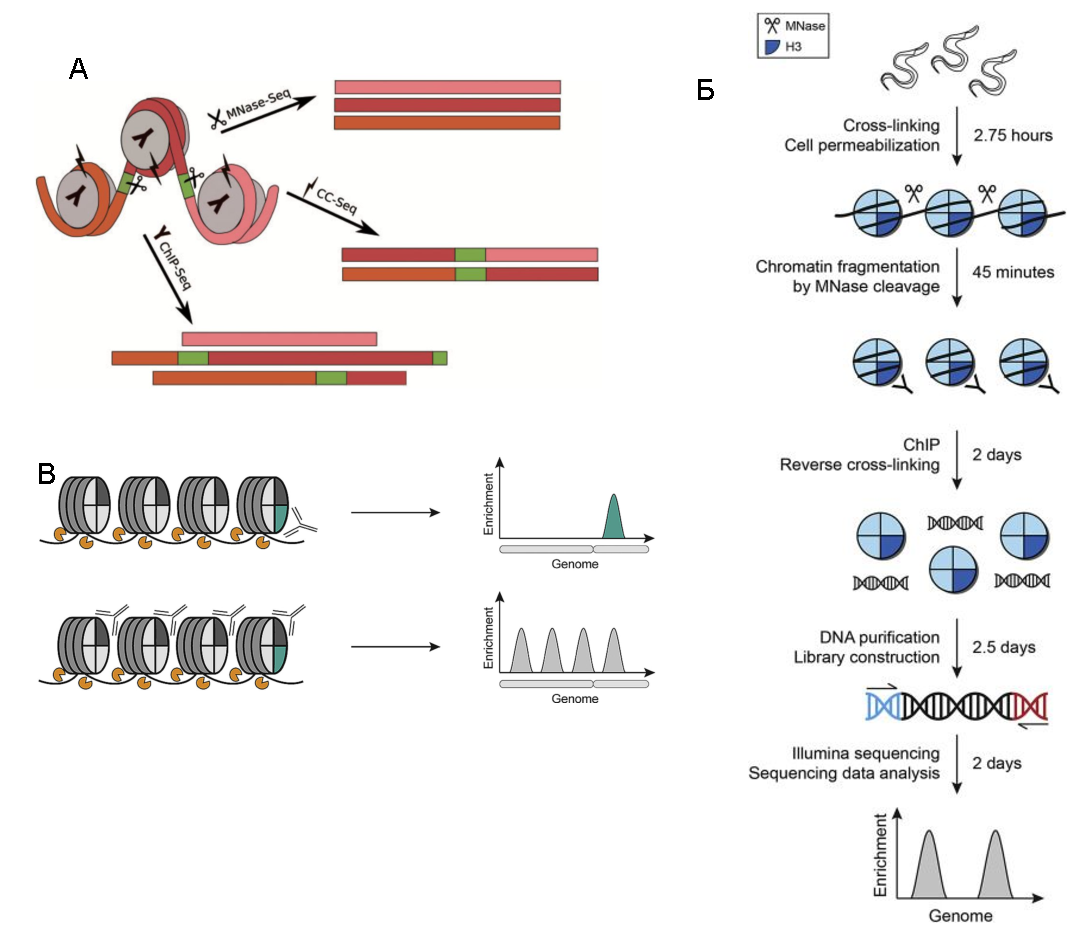
\includegraphics [width=\textwidth]{images/p1/part1_5_genome/p1_5_genome_f6.pdf}
    \caption[Методы эпигеномики нуклеосомного разрешения]{Методы эпигеномики нуклеосомного разрешения: А) MNase-seq, ChIP-seq, CC-seq. Б-В) MNase-ChIP-seq. Адаптировано из \cite{quintales_comparative_2015} и \cite{wedel_genome-wide_2017}.}
    \label{fig:p1_5_genome:f6}
\end{figure}
















